\documentclass[12pt]{article}
\usepackage[margin=1in]{geometry}
%\usepackage[letterpaper, margin=1in, left=1in]{geometry}
\usepackage[T1]{fontenc}
\usepackage[utf8]{inputenc}
\usepackage{times}
\usepackage[english]{babel}
\usepackage{wrapfig}
\usepackage[pdftex]{graphicx}
\usepackage{caption}
\usepackage{sectsty}
\usepackage{titling}
\usepackage{titlesec}
\usepackage[normalem]{ulem}
\usepackage{color,soul}
\usepackage{epstopdf}
\usepackage{natbib}
\usepackage{lineno}
\usepackage{booktabs}
\usepackage{longtable}
%\setcitestyle{numbers} 
%\bibliographystyle{vancouver}
\bibliographystyle{natbib}
\setlength{\bibsep}{0pt}
\usepackage{graphicx}
\titleformat{\section}{\bfseries\fontsize{11}{12}\selectfont}{\thesection}{1em}{}
\renewcommand{\thesection}{\Roman{section}} 
\titleformat{\subsection}[runin]{\itshape\bfseries\fontsize{11}{12}\selectfont}{}{}{}[~~]
\titleformat{\subsubsection}[runin]{\itshape\fontsize{11}{12}\selectfont}{}{}{}[~~]
\titlespacing*{\section}{0pt}{5pt}{0pt}
\titlespacing*{\subsection}{0pt}{5pt}{0pt}
\titlespacing*{\subsubsection}{0pt}{5pt}{0pt}

\bibpunct{(}{)}{;}{a}{}{,}
\makeatletter
\newcommand\iraggedright{%
      \let\\\@centercr\@rightskip\@flushglue \rightskip\@rightskip
        \leftskip\z@skip}
\makeatother

\iraggedright

\captionsetup{%
   justification=raggedright,
   labelfont=bf,
   textfont=bf}
\linespread{2}
\pagenumbering{arabic}
%\allsectionsfont{}
%\subsectionfont{}
\linenumbers
\begin{document}

\setcounter{page}{1}

\noindent \textbf{Running head:} PLACING FOSSILS WITH MORPHOMETRIC DATA

\noindent \textbf{Title:} Bayesian and likelihood placement of fossils on phylogenies from quantitative morphometrics

\noindent Caroline Parins-Fukuchi

\noindent {\it Department of Ecology and Evolutionary Biology, University of Michigan, Ann Arbor, Michigan, 48109, USA.}

\noindent E-mail: cfukuchi@umich.edu

\noindent Telephone: (734) 474-7241

\medskip

%\medskip

%\vspace{1in}
\newpage

\noindent \textbf{\textsc{Abstract}}

Jointly developing a comprehensive tree of life  from living and fossil taxa has long been a fundamental issue in evolutionary biology. Broad questions, including reconstruction of species relationships, comparative patterns, and divergence times can  benefit from an integration of information gleaned from neo- and paleontological viewpoints. One major limitation has stemmed from difficulties in merging evidence  from extant organisms, from which molecular data can be extracted, and extinct organisms, which are only known from morphology and stratigraphy.  While many fields have reached varying stages of synthesis between fossils and DNA, these efforts have been hindered by the qualitative descriptions of morphological characters typically employed in phylogenetic analyses. Although they have rarely been applied to phylogenetic inference, morphometric methods can improve these issues by generating more rigorous ways to quantify variation in morphological structures, and have the added benefit of facilitating the rapid and objective aggregation of large morphological datasets. In this paper, I describe a new Bayesian method to that analyzes  geometric or traditional morphometric data to identify the positions of fossil taxa on reference trees. This method includes a formulation of the phylogenetic Brownian motion model that reconstructs branch lengths based on morphological disparity that do not require scaling to absolute time scale. This relaxation of the need to infer an absolute timescale can facilitate a new framework though which to construct true Bayesian node calibration priors for molecular dating that directly incorporate uncertainty derived from the analytical placement of fossils and may also offer a new option through which to explore patterns in morphological disparity across taxa that simplify existing phylogenetic comparative methods. Generally, I am hopeful that the approach described here will help to facilitate a deeper integration of neo- and paleontological data to move morphological phylogenetics further into the genomic era.


\noindent {\bf Keywords:} phylogenetics, morphology, paleontology, quantitative characters, Bayesian

\subsection*{Acknowledgements}
I  thank James Saulsbury, Joseph Walker, and Stephen Smith for helpful comments that improved the manuscript. 

\subsection*{Supplementary Data}
All supplemental material, including scripts, newick files, morphological and molecular alignments used in this study are available as a GitHub repository (https://github.com/carolinetomo/fossil\_placement\_tests). 	

\newpage

\noindent\textbf{Introduction:} The role of fossil data in reconstructing
phylogeny among living organisms has long been a central, yet
contentious, topic in evolutionary biology. This has manifested over the past decade
in the rapid proliferation of 'total-evidence' methods that seek to simultaneously reconstruct the relationships
and divergence times between living and fossil taxa using cladistic morphological matrices.
 These approaches, based upon probabilistic models of molecular and
morphological character, have increased understanding of evolutionary tempo across large clades,
and provide compelling evidence in favor of incorporating fossils in
phylogenetic analyses \citep{pyron2011divergence,ronquist2012total}.

Researchers' enthusiasm for reconstructing a comprehensive tree of life
has encouraged the integration of fossils with living taxa in
phylogenetic analyses. Improving integration between fossil and living
taxa has the capability to benefit both paleo- and neontological
studies. In addition to the results of Berger and Stamatakis discussed
above, the inclusion of fossils improves the reconstruction of ancestral
states using phylogenetic comparative methods \citep{slater2012integrating}. As
another example, increasing the rigor with which fossils are placed on
phylogenies is expected to improve the accuracy and treatment of
uncertainty in divergence time estimation \citep{guindon2018accounting}.

A constant source of difficulty when jointly estimating phylogeny between living
and extinct organisms is the unavailability of molecular data in nearly
all fossil taxa. As a result, there has been a need to explore the
compatibility of molecular with morphological data to better understand
the capability of fossil and extant species to reciprocally inform
reconstruction of phylogeny and divergence times. Previous work has
sought to determine whether the inclusion of molecular data representing
extant species can improve the reconstruction of relationships among
fossils represented by morphology alone \citep{wiens2009paleontology,wiens2010combining}. The result
of these studies suggest that the inclusion of morphological characters
comprising living and fossil species does not have a tendency to
decrease the accuracy of phylogenetic reconstructions, and can improve
estimation of fossil placements in well-behaved datasets. Expanding upon
these observations, \cite{berger2010fossilplacement} have shown that methods
placing fossils on fixed molecular phylogenies can yield accurate
results by filtering through conflicting signal. This shows
that placing incomplete fossil data in a molecular context scaffolded by
extant relationships can improve reconstruction among fossils.


Despite the abundance of both clear and subtle benefits to improving the
integration of fossil and living taxa in phylogenetics, challenges have
arisen from conflicting and noisy information presented by morphological
data. Another issue that is noted by Berger and Stamatakis (cited above) stems from the reality that
morphological alignments commonly contain very few sites, often 50-500,
compared to molecular datasets, which can contain hundreds of thousands
of sites. This can cause the likelihood of molecular partitions to dwarf
those of morphological partitions, limiting the influence of morphology
in reconstructions of topology and branch lengths. For these reasons,
Berger and Stamatakis advocated fixing the relationships of extant taxa
\emph{a priori} using molecular reconstructions, and using the resulting
scaffold to identify conflicting signal in morphological data.

The fragmentary nature of fossil data further exacerbates these challenges.
 These occur at multiple levels important to phylogenetic analysis. At one level, morphological data are frequently susceptible to
displaying biased or misleading signal. This may often stem in part from
the general practice of assigning discrete character states to taxa
through qualitative assessment. The subjective nature of this process
can cause major irreconcilable disagreement between results achieved
from different researchers \citep{hauser1991effect,pleijel1995character,wilkinson1995comparison,
hawkins1997primary,scotland2000homology,scotland2003phylogeny,brazeau2011problematic,simoes2017giant}. As an added layer of
potential bias, these matrices are also frequently filtered to include
only characters that researchers consider before the fact to be
accurately informative in phylogenetic reconstruction. At another level,
the discrete character matrices most commonly employed in phylogenentics
can often be difficult to adequately model. At present, researchers
employing probabilistic methods generally use the so-called `Mk' model
\citep{lewis_mk}. This is a generalization of the Jukes-Cantor model of
nucleotide substitution that accommodates \emph{k} possible character
states. Although previous work based upon simulated data has suggested
that Mk-based approaches outperform parsimony \citep{wright2014bayesian},  the extent and conditions under which this is the
case in empirical datasets is unclear (Goloboff et al.~2017). Empirical
datasets are also likely to depart significantly from the assumptions of
the Mk model.  This poor match between model assumptions and data  can lead to erratic results and high uncertainty in
posterior estimates of divergence times \citep{ronquist2016closing}. The sensitivity of topological reconstruction to this frequent mismatch is fairly unclear at present. 

For all of these reasons, continuous traits have been suggested as a
feasible alternative \citep{felsenstein1973,felsenstein1988phylogenies,macleod2002phylogenetic,parins2017use}. Tools that quantify morphological size and shape have the capacity to alleviate many of the concerns relating to bias and
subjectivity that occur with discrete characters. Approaches such as
geometric morphometrics offer the potential to holistically incorporate
all dimensions of shape to inform phylogeny. The continuous state space
of morphometric data might also increase the amount of information that
can be extracted from morphological datasets, which may be beneficial
when analyzing poorly-sampled fossil data.

Traditional linear morphometric measurements have long been employed in
morphological phylogenetics, but are typically discretized to more
easily analyze them alongside present-absence data. However, these
transformations may decrease the amount of information in continuous
datasets by binning fine-scaled variation into shared discrete
categories, and are susceptible to the difficulties in modeling under
the Mk model described above. Geometric morphometric data have shown
utility in several previous phylogenetic studies using parsimony-based
methods \citep{geomorphhominin,catalano2010phylogenetic,smith2013geometric}, but have not gained substantial traction.
This may be in part due to the lack of available tools to analyze
continuous trait data in a probabilistic framework.

The earliest studies investigating probabilistic methods of phylogenetic
inference were developed using continuous characters modelled under
Brownian Motion (BM) \citep{cavalli1967,felsenstein1973}. Due in part to the abundant discrete character data that became
available with the emergence of DNA sequencing, these approaches were
quickly overshadowed in popularity by discrete trait approaches based
upon Markov nucleotide substitution models. Continuous trait models have
since gained significant popularity in phylogenetic comparative methods,
but still are rarely used for phylogenetic inference. As a result, few
implementations exist, with only ContML in the PHYLIP package and
RevBayes (through scripting) providing such functionality \citep{hohna2016revbayes}. The
approaches used in these packages are also fairly minimalistic, with no
real tailoring to the challenges that might be presented by empirical
datasets.

In this paper, I describe a new approach that places fossils on
molecular trees using quantitative characters modeled under BM. This
 seeks to tackle some of the most pressing obstacles associated
with the use of traditional and geometric morphometric data in
phylogenetic inference. Using simulated data, I validate and explore the
behavior of the implementation. I also analyze empirical datasets
representing the Vitaceae family of flowering plants (citation?) and carnivoran
mammals \citep{jones2015impact} comprised of traditional and geometric
morphometric measurements, respectively. The method uses Markov chain
Monte Carlo (MCMC) to infer the evolutionary placements of fossils and
branch lengths. Although MCMC is generally associated with Bayesian
inference, the implementation described here can perform inference both with and without
the use of priors to enable exploration of a range of inferential paradigms to best accommodate diverse
morphometric datasets.

\noindent\textbf{Methods and Materials:}

\noindent\emph{Brownian motion model}

The approaches that I describe in this paper all rely upon the familiar
BM model of evolution \citep{butler2004phylogenetic,o2006testing} . Under BM, traits are assumed to be multivariate
distributed, with variances between taxa defined by the product of their
evolutionary distance measured in absolute time and the instantaneous
rate parameter ($\sigma$):

\begin{equation}
 dX(t) = \sigma dB(t)
\end{equation}

where \emph{dX(t)} is the time derivative of the change in trait
\emph{X} and \emph{dB(t)} corresponding to normally distributed random
variables with mean 0 and variance \emph{dt}. This leads to the
expectation that over time \emph{t},

\begin{equation}
 E(X_t) = X_0 
\end{equation}

with

\begin{equation}
Var(X_t) =  \sigma t
\end{equation}


where $X_0$ gives the trait value at $t_0$.

The methods that I describe use a slightly different parameterization
and likelihood calculation than most conventional implementations used
in modern phylogenetic comparative methods (PCMs). These generally
construct a variance-covariance (VCV) matrix from a dated, ultrametric
phylogeny to calculate the likelihood of the data, assuming a
multivariate normal distribution \citep{butler2004phylogenetic,o2006testing}. Since these methods treat the topology and
branching times as known, the goal is typically to obtain the maximum
likelihood estimate (MLE) of the rate parameter ($\sigma$ ) to examine
evolutionary rate across clades.

One drawback to the use of this version of the phylogenetic BM model in
the reconstruction of topology is its requirement that phylogenies be
scaled to absolute time. Although it is possible to simultaneously
estimate divergence times and topology while analyzing continuous
traits, this can cause additional error and requires the specification
of a tree prior that can accommodate non-ultrametric trees that include
fossils. This requirement would also cause circularity in cases where
researchers are interested in obtaining estimates and error in fossil
placements in order to more rigorously inform molecular clock
calibrations. To overcome the need for simultaneously estimating
divergence times and fossil placements, I estimate the product
$\sigma t$ together. As a result, rate and absolute time are
confounded in the trait and tree models. Branch lengths, which reflect the morphological disparity
between taxa, are thus measured in units of morphological standard
deviations per site. This interpretation could be thought roughly of as
a continuous analogue to the branch lengths obtained from discrete
substitution models. Similarly to the discrete case, long branch lengths
could reflect either a rapid rate of evolution or a long period of
divergence (in absolute time) along that lineage.

\noindent\emph{Computation of the likelihood:}

Rather than use the computationally expensive VCV likelihood
calculation, I use the reduced maximum likelihood (REML) calculation
described by Felsenstein (1973). In this procedure,  the tree likelihood is computed  from the
phylogenetic independent contrasts (PICs) using a `pruning' algorithm. In this procedure, each internal node is visited in a postorder traversal, and the log- likelihood, $L_{node}$ is calculated  as multivariate normal, with a mean equal to the contrast between the character states, $x_1$ and $x_2$ at each subtending edge  and variance  calculated as the sum of each child edge, $v_1$ and $v_2$:

\begin{equation}
L_{node} = \frac{1}{2}*\frac{\log{(2\pi)}+\log{(v_1+v_2)}+(x_1-x_2)^2}{v_1+v_2}
\end{equation}

\noindent  The PIC, $x_internal$, is  calculated at each internal node and used as the character state representing the internal node during the likelihood computation at the parent node. The edge length of the internal node, $v_internal$ is also extended by averaging the lengths of the child nodes to allow the variance from the tips to propagate from the tips to the root:

\begin{equation}
x_{internal} = \frac{(x_1*v_2)+(x_2*v_1)}{v_1+v_2}
\end{equation}

\begin{equation}
v_{internal} = v_{internal} + \frac{(v_1*v_2)}{(v_1+v_2)}
\end{equation}

\noindent This procedure is performed at each internal node. The total log-likelihood of the tree, $L_{tree}$ is calculated by summing the log-likelihoods calculated at each of the $n$ internal nodes.

\begin{equation}
L_{tree} = \sum\limits_{node=1}^{n} L_{node}
\end{equation} 

\noindent\emph{Priors:}

Since the estimation of branch lengths from continuous traits is
relatively uncharted territory in phylogenetics, I implemented and
tested three different branch length priors derived from the molecular
canon: 1) flat (uniform), 2) exponential, and 3) a compound dirichlet
prior after  \citep{rannala2011tail}. The compound dirichlet prior also
offers an empirical Bayes option that uses an initial ML estimate of the
branch lengths to specify the parameter corresponding to mean tree
length.

\noindent\emph{Markov-chain Monte Carlo}

 This method uses a
 Metropolis-Hastings (MH) algorithm \citep{hastings1970monte} to simulate the posterior or confidence distribution of fossil insertion points
and branch lengths. Rearrangements of the topological positions of fossil taxa are performed by randomly pruning
and reinserting a fossil taxon to generate a proposal. This is a
specific case of the standard subtree pruning and regrafting (SPR) move
for unrooted tees. Branch lengths are updated both individually and by randomly applying a
multiplier to subclades of the tree. MH proposal ratios were derived from the unrooted SPR and multiplier moves described by \cite{yang2014molecular}.

\noindent\emph{Generating a rough ML starting tree:}

To generate an initial estimate of fossil placements and branch lengths,
I estimate an approximate ML starting tree. Initial placements are
achieved using stepwise addition. Each fossil is individually inserted
along all existing branches of the tree, with the insertion point that
yields the highest likelihood retained. At each step, MLEs of the branch
lengths are computed using the iterative procedure introduced by
\citep{felsenstein1981evolutionary}. In this procedure, the tree is rerooted along each
node. PICs are calculated to each of the three edges subtending the new
root, and then the MLE of each edge ($v_i$) is computed analytically
by averaging the distances between the PICs calculated from each
\emph{j} of \emph{n} sites in the character alignment ($x_{ij}$):

\begin{equation}
 \hat{v_{1j}} =   \frac{\sum\limits_{j=1}^{n}(x_{1j}- x_{2j}) (x_{1j} - x_{3j}) }{n}
\end{equation}

\begin{equation}
 \hat{v_{2j}} =   \frac{\sum\limits_{j=1}^{n}(x_{2j}- x_{1j}) (x_{2j} - x_{3j})}{n} 
\end{equation}

\begin{equation}
\hat{v_{3j}} =   \frac{\sum\limits_{j=1}^{n}(x_{3j}- x_{1j}) (x_{3j} - x_{2j})}{n}
\end{equation}


This process is iterated by successively rerooting on each node of the
tree and calculating the branch lengths until their values and the
likelihoods converge. Felsenstein (1981) gives a more detailed
explanation of the algorithm, along with a complete derivation of the
three-taxon MLEs.

Once the optimal placement of all of the fossils has been identified,
the branch lengths are recalculated and can be used to inform branch
length priors used during MCMC simulation. One problem with interpreting
the results of the ML approach on their own is that it has a strong
propensity to becoming trapped in local optima. As a result, it should
be used and interpreted cautiously in  messy datasets. In the
applications here, the topologies achieved from this procedure are
restricted to the construction of starting trees, while the branch
lengths inform the specification of branch length priors. This procedure
allows straightforward construction of non-random starting trees for the
MCMC and priors that reflect the the dataset under analysis.

\emph{Filtering for concordant sites:}

One major hurdle involved in the use of morphological data is their
frequent tendency to display noisy and discordant signal. This problem
might be expected to manifest even more intrusively in morphometric
datasets than in discrete datasets, since traits are much less likely to
be excluded \emph{a priori} on the basis of perceived unreliability. As
a result, there is a need to filter through noisy signal to favor more
reliable sites. I developed a procedure adapted from Berger and
Stamatakis (2010) for this purpose. This computes a set of weights based
upon the concordance of each site with the reference tree. In this
procedure, the likelihood (\emph{L}\textsubscript{ref}) of each site is calculated on
the reference tree (excluding fossil taxa). Next, the likelihood
(\emph{L}n) of each site is calculated along each \emph{n} of 100
randomly generated phylogenies. If the likelihood of the site is higher
along the reference tree than the current random tree, the weight of the
site is incremented by one. Thus, site \emph{j} receives the integer
weight:

\begin{equation}
\overrightarrow{W}^{int}_j = \sum\limits_{n=1}^{100}\delta_n 
\end{equation}

where $\delta nj$ = 1 if:

\begin{equation}
L_{ref} > L_n 
\end{equation}

and $\delta nj$ = 0 if:

\begin{equation}
L_{ref} < L_n 
\end{equation}

This yields a weight vector that is the same length as the character
matrix, with each site possessing a weight between 0 and 100. The sites
are then weighted using one of three schemes: 1) whole integer values,
where the weight equals the value obtained from equation 7, 2) a
floating point value between 0 and 1, where the value generated from the
random comparison is divided by 100, and 3) a binary value where the
weight is equal to 1 if the site displayed a higher likelihood in the
reference tree than 95 or more of the random trees, and 0 if less than
95:

\begin{equation}
\overrightarrow{W}^{binary}_j = 1
\end{equation}

if 

\begin{equation}
\overrightarrow{W}^{int}_j > 95 
\end{equation}

and

\begin{equation}
\overrightarrow{W}^{binary}_j = 0
\end{equation}

if

\begin{equation}
\overrightarrow{W}^{int}_j <  95
\end{equation}

In application, I found that integer weighting caused poor MCMC mixing,
and so the floating and binary schemes are probably most practical in
most cases. Since it filters out discordant sites completely, the binary
scheme is enforces a harsher penalty than the floating and integer
schemes, and so might be of greatest use in particularly noisy datasets.
As an additional note, although these procedures share similar
terminology to the site weights calculated during parsimony analysis of
multi-state characters, they differ in their purpose. Parsimony site
weights are intended to normalize the contribution of characters with
differing state spaces to the overall tree length. In contrast, the site
weighting approach deployed here is designed to decrease the
contribution of sites that disagree with the reference topology to the
overall tree likelihood, instead highlighting signal that is taken to be
more reliable. As a result, the guide tree is used to identify sites
that are most likely to reliably inform fossil placements.

\noindent\emph{Simulations:}

To explore the behavior of these approaches under different settings and
to validate the implementation, I performed a set of simulations. From a
single simulated tree, I pruned five ``fossil'' taxa and
estimated their positions along the tree using 100 datasets of 50
characters simulated under BM. The tree was simulated under a
birth-death model, with a birth parameter of 1.0 and a death parameter
of 0.5. Extinct lineages were retained. The final tree conained 41 taxa,
leaving a 36-taxon reference tree when the five fossils were pruned. To
explore the effect of conflicting and noisy signal, I also generated
alignments consisting of 50 ``clean'' traits simulated along the true
tree, and combined with partitions of ``dirty'' traits in intervals of
10, 25, and 50 generated along random trees. All simulations were
performed using the phytools package \citep{revell2012phytools}.

I restricted the simulations to a fairly small number of traits because
this reflected a similar alignment size as the two empirical datasets.
This level of sampling is fairly common among existing morphometric
datasets, which are typically compiled from only one or two organs. In
the future, I am hopeful that quantitative morphometric datasets will
increase in size to encompass much broader sampling across organs, but
at present, it seemed most sensible to examine the level of sampling
expected from existing datasets. Unlike in a previous paper
(Parins-Fukuchi 2017), I also did not simulate traits that display
covariance among sites. This is because 1) I show in the previous study
that covariance does not significantly handicap reconstructions from
continuous traits, and 2) because in this study I was primarily
interested in examining the effect of inducing random noise without the
potentially confounding effect of covariance. Although covariance has
been expressed as a major concern in morphometric phylogenetics
\citep{felsenstein1988phylogenies,felsenstein2002quantitative}, there is no reason to expect greater
covariance between continuous traits than discrete traits, which,
ideally, should describe similar aspects of morphology.

These simulated datasets were then used to reconstruct the placements of
the five fossils. To explore the relative performance of weighting
schemes, I performed reconstructions using both the binary and floating
approaches. These were supplemented by analyses of the noisy datasets
without applying site weights. MCMC simulations were run for 1,000,000
generations and checked to ensure that the effective sample sizes (ESS)
exceeded 200. The exponential branch length prior was employed for the
simulated data with a mean of 1.0. To evaluate the accuracy of the
placement method, I then calculated the distances between the true and
reconstructed fossil placements. This was calculated by counting the
number of nodes separating the true insertion branch from the
reconstructed insertion branch. Placement accuracy was evaluated using the
\emph{maximum a posteriori} (MAP) summaries of tree distributions. MAP
trees represent the single most sampled tree during the MCMC run. They
are thus somewhat analogous to ML trees in presenting the point estimate
that is assumed to have the highest asymptotic density over the
likelihood or posterior (depending on paradigm) surface. Clade support
values were also calculated. Tree summary and placement distances
were calculated using custom Python scripts.

\noindent\emph{Empirical analyses:}

I estimated the phylogenetic positions of fossils using a morphological
matrix comprised of 51 continuous measurements gathered from pollen and
seed specimens sampled across 147 extant and 8 fossil Vitaceae taxa.
These data were acquired from Chen (2009). I constructed a guide tree
for the extant taxa from 8 nuclear and chloroplast genes gathered from
Genbank using the PHLAWD system \citep{soltis2011angiosperm}.
 Using this scaffolding, I analyzed the morphological data to estimate the positions of the fossil taxa.
Individual runs were performed under all three branch length priors to
assess stability across models. All analyses were run for 30,000,000
generations and visually checked for convergence. Analyses were
performed with binary weights applied to the sites and compared to an
unweighted analysis. To ensure that MCMC runs were not trapped in local
optima, several runs were performed under each combination of settings.
For each, the analysis with the highest mean likelihood was retained.

To explicitly test the informativeness of geometric morphometric data in
fossil placement, I also performed analyses on a dataset of 33 3D landmark
coordinates representing 46 extant and 5 extinct fossil carnivoran
crania \citep{jones2015impact}. A reference tree composed of the 46 extant
taxa was obtained from the data supplement of the original study. These
coordinates were subjected to Procrustes transposition using MorphoJ \citep{klingenberg2011morphoj}.
This yielded a matrix where each character represented the X, Y, or Z position of one landmark.
The resulting traits displayed phylogenetic signal, but the transformed
coordinates showed very low dispersion (variance) on an absolute scale.
This appeared to flatten the likelihood surface, causing difficulites in
achieving MCMC convergence. To remedy this, I scaled all of the traits
to increase the absolute variance evenly across taxa evenly at each site while
maintaining the original pattern of relative variances across taxa using the scale() function in R \citep{R}. This
procedure preserved the signal present in the original dataset, since the
relative distances between taxa remained the same. Final analyses were
performed on this transformed set of measurements. As with the
Vitaceae dataset, I analyzed the canid data under all three branch
length priors. MCMC simulations were run for 20,000,000 generations, and
visually examined using Tracer v1.6 to assess convergence. Both
empirical datasets achieved large ESS values.

For both datasets, I used starting trees and branch lengths generated
from the rough ML method described above. Sites were weighted using the
binary for the final analyses. Intermediate analyses using unweighted
and float-weighted sites were also performed, and are presented in the
data supplement. Dirichlet priors were assigned alpha parameters of 1.0
and beta parameters specified as the total tree length of the ML
starting tree. Exponential branch length priors were assigned mean
values of 1.0.

Since the empirical datasets were more complex than the simulated data,
I summarized the tree distibutions as maximum clade credibility (MCC)
summaries. These summaries maximize the support of each clade. These
were compared to the MAP estimates, however, and yielded generally
concordant placements (supplementary material). MCC summaries were
obtained using the SumTrees script that is bundled with the DendroPy
package \citep{sukumaran2010dendropy}. Branch lengths were summarized as
the mean across all sampled trees.

\noindent\emph{Software:}

All analyses of fossil placements and branch lengths were performed
using the new software package \emph{cophymaru} written in the Go
language. The source code is publicly available as free software at
https://github.com/carolinetomo/cophymaru.

\noindent\textbf{Results and Discussion}

\noindent\emph{Simulations}

Reconstructions of fossil placements from the simulated datasets showed
that the method is generally accurate in placing fossil taxa (Table 1).
In the absence of noisy traits, reconstruction is nearly always correct,
with the reconstructed position of each fossil placed less than 0.1
nodes away from the true position on average. In the presence of random
noise, the reconstructions are fairly accurate, except when noise
becomes severe. Nevertheless, even in extreme cases, estimated positions
tend to fall within the correct region of the tree, falling 1.85 and
\textasciitilde{}3 nodes away from the correct placement on average when
alignments contain an equal number of clean and dirty sites.

Overall, binary weighting shows improved accuracy over float and
unweighted analyses. However, despite the apparent advantage of binary
weighting, it is possible that the float weighting scheme could remain
beneficial in cases where the distribution of noise varies betwen
different regions of trees. This is because the float weighting scheme
limits the contribution of noisy sites to the likelihood rather than
entirely excluding them. This possibility was not examined in this set
of simulations, since the dirty traits were generated to reflect
completely random noise. However, in reality, noise may be structured to
display . In these cases, continuous traits may display misleading
signal among some subset of taxa, but correctly informative signal among
other subsets. Further work will be needed to determine whether absolute
float weight values scale predictably with the noisiness of particular
sites across clades.

Overall, the simulations demonstrate the efficacy of the method for the
phylogenetic placement of fossils and provide a validation of the
computational implementation. The analysis of clean datasets shows that
the method performs well, estimating fossil placements with very low
error when signal is clear. The adaptation of Berger and Stamatakis'
(2010) site weight calibration approach also appears to effectively
filter through noisy datasets to improve estimation. The binary weight
calibrations appear particularly effective at dealing with rampant
misleading random noise, with improving accuracy by 2 to 20 times
depending on the relative proportion of signal and noise compared to
unweighted analyses. These results show promise toward the prospect of
applying the method developed in this work to the analysis of
large-scale morphometric datasets, where significant noise might be
expected. Although introducing noise to unweighted analyses decreases
reconstruction accuracy, the method performs predictably, and still
manages to place fossils on average within the correct neighborhood.
However, when weighting schemes are applied, the performance improves
drastically, highlighting the promise of this method for the analysis of
empirical datasets.

\begin{longtable}[]{@{}llll@{}}
\toprule
dataset & binary\_weights & float\_weights & unweighted\tabularnewline
\midrule
\endhead
50 clean & 0.065 & 0.067 & 0.059\tabularnewline
50 clean + 10 dirty & 0.156 & 1.234 & 2.516\tabularnewline
50 clean + 25 dirty & 0.965 & 2.623 & 3.105\tabularnewline
50 clean + 50 dirty & 1.85 & 3.069 & 3.348\tabularnewline
\bottomrule
\end{longtable}

\textbf{Table 1.} Mean distances of true and reconstructed fossil
placements. Distances are measured as the average number of nodes
separating reconstructed placements from their true positions across all
100 replicates of each dataset.

\noindent\emph{Vitaceae dataset:}

Application of the fossil placement method to the Vitaceae dataset
showed generally positive results. The weight calibration procedure
revealed substantial noise in the dataset, with 10-12 of 51 sites
failing to favor the molecular reference tree over the random trees at
least 95\% of the time across all runs. Despite this noise, the binary
weighting scheme appeared to adequately filter through this noise to
generate biologically reasonable results. \emph{Vitis tiffneyi},
\emph{Parthenocissus\_clarnensis} , and \emph{Ampelopsis rooseae} all
share clades with the extant members of their respective genera.
\emph{Palaeovitis\_paradoxa}, and \emph{Cissocarpus jackesiae}, which
represent genera with no extant species, both group confidently with
separate, non-monophyletic groups of crown \emph{Cissus}.
\emph{Ampelocissus wildei} is placed convidently along with crown
\emph{Cissus}, separated by only a node from \emph{Palaeovitis
paradoxa}. All six of these taxa are stable in their placements,
grouping within the same clades across runs, and when both the
exponential and empirical compound dirichlet priors are applied.

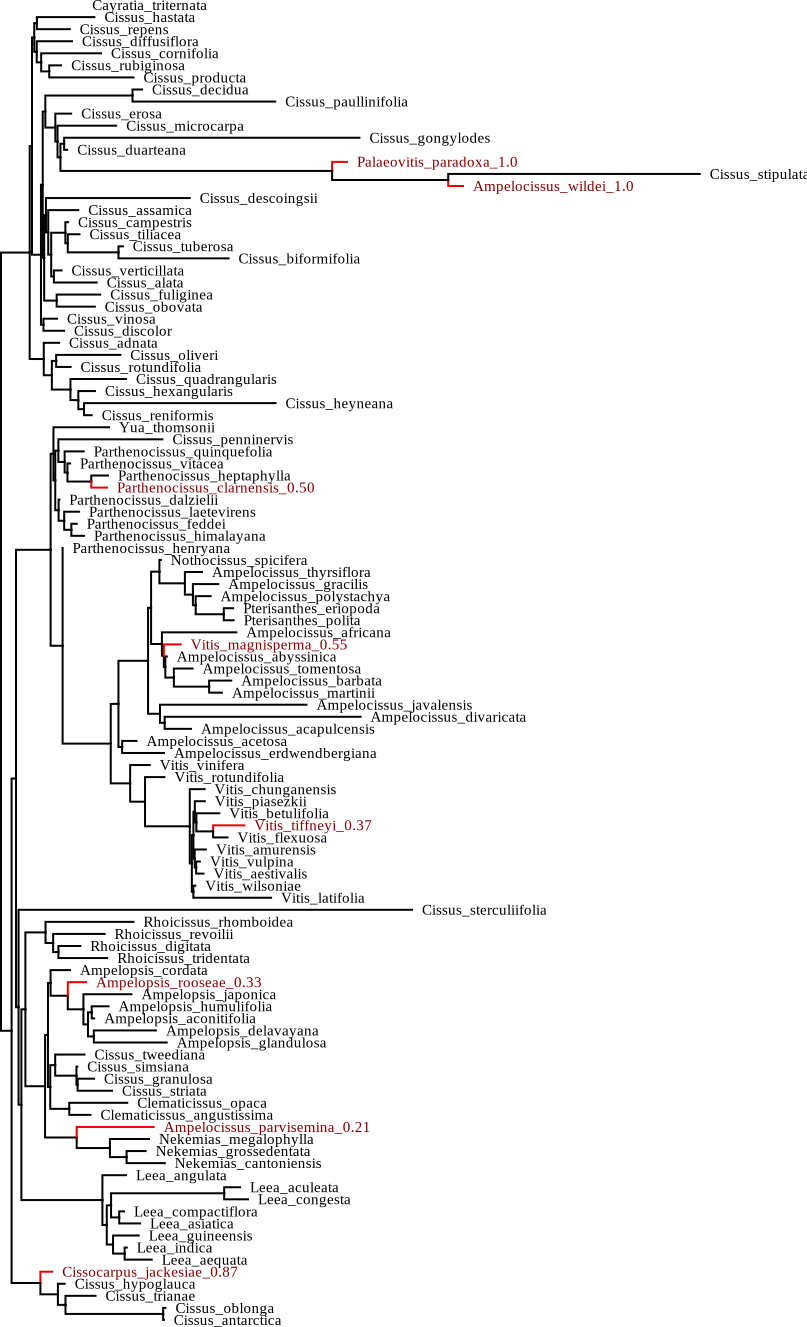
\includegraphics[width=\textwidth,height=\textheight]{/home/tomo/projects/fossil_placement/vitfig.pdf}

\textbf{Figure 1.} Vitaceae fossil placements inferred under the
exponential branch length prior. Fossil taxa and branches are
highlighted in red. Values following fossil tip labels indicate
posterior support for placement. Topology is summarized from the
posterior using the set of maximally credible clades (MCC). The placements are depicted only in the subclade containing all 6 fossils.

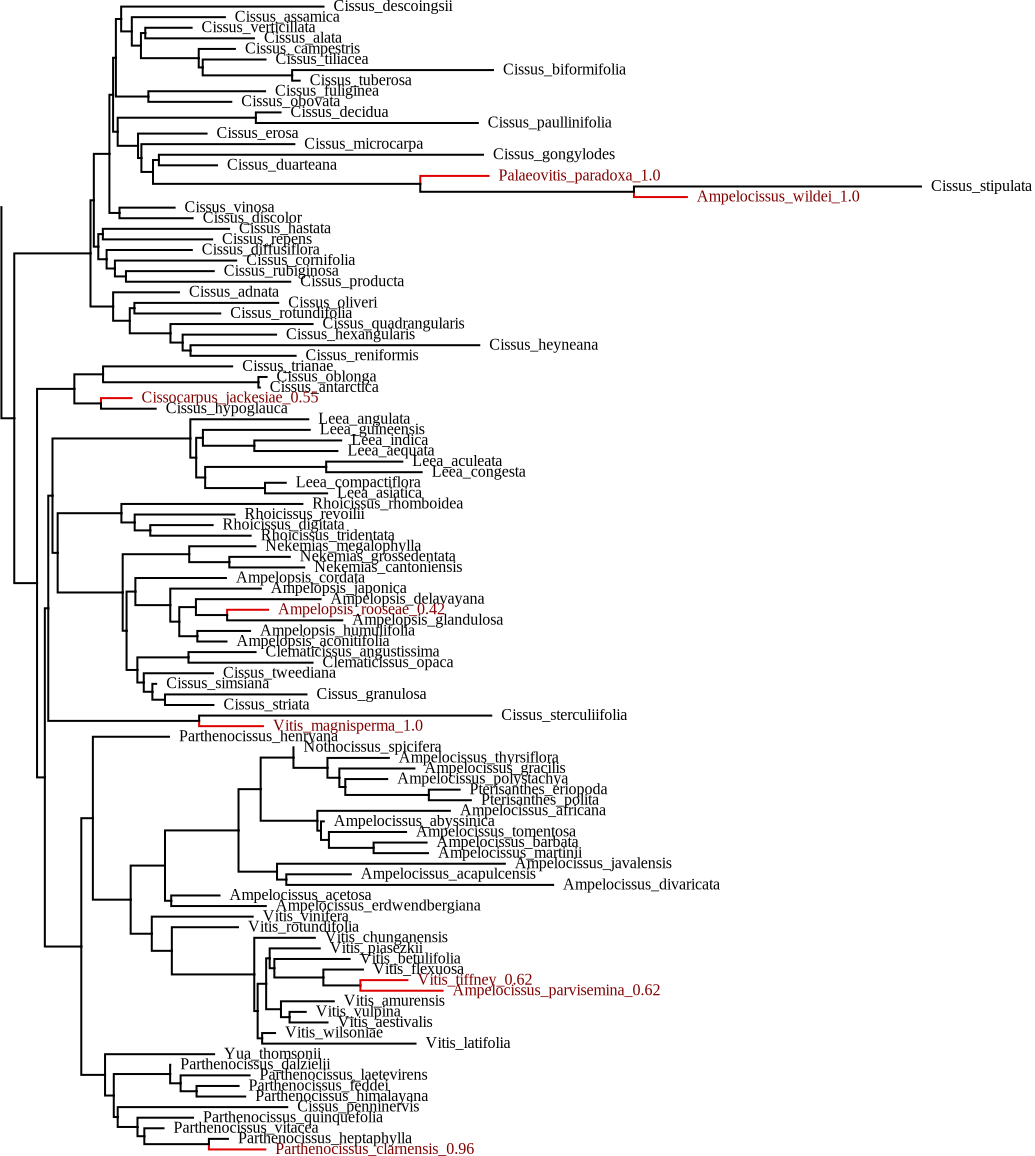
\includegraphics[width=\textwidth,height=\textheight]{/home/tomo/projects/fossil_placement/vitfigdirichlet.pdf}

\textbf{Figure 2.}  Vitaceae fossil placements inferred
under the compound dirichlet branch length prior. Fossil taxa and
branches are highlighted in red. Values following fossil tip labels
indicate posterior support for placement. Topology is summarized from
the posterior using the set of maximally credible clades (MCC). The placements are depicted only in the subclade containing all 6 fossils.

The remaining two fossils are substantially less stable in their
placements. \emph{Ampelocissus parvisemina} shows erratic placement,
alternately occupying clades shared by crown \emph{Vitis} or
\emph{Nekemias} in the best exponential and dirichlet prior runs,
respectively. Its placement also changes across different runs using the
same prior, and shows poor support in all cases. Under the exponential
prior, the \emph{Ampelocissus parvisemina} placement shows a 0.2
posterior probability, which decreases to 0.058 under the dirichlet
prior. Similarly, \emph{Vitis magnisperma} alternately resolves into
clades shared by crown \emph{Cissus} and \emph{Ampelocissus} under the
exponential and dirichlet priors, with posterior support values of 0.23
and 0.54, respectively.

Despite the  erratic behavior of the last
two taxa, the low posterior support exhibited by their placements is
reassuring. In many cases, fossils may simply present weak information
due to shortcomings in geologic and taxonomic sampling. When this is
occurs, it is unlikely that any greater certainty in their placement can
be achieved except with increased data. Therefore, one major benefit to
the approach described here is the clarity with which it
describes uncertainty in the placement of fossils. Importantly, such
uncertainty revealed by analysis under this method may improve the
utility of erratic fossils. For instance, while such fossils are often
omitted from analysis due to perceived unreliability, this approaches
described here demonstrate more clearly the confidence and uncertainty
surrounding a reconstructed set of possible placements. This uncertainty
may allow the fossils to participate in node calibration for molecular
dating using new methods that accommodate uncertainty in calibration
placement \citep{heath2014fossilized,guindon2018accounting}. Since the present analyses
quantify the uncertainty in fossil placements, this information may be
used to construct non-arbitrary, true Bayesian priors on node ages.

\noindent\emph{Carnivoran dataset:}

Analysis of the carnivoran dataset also yielded generally reasonable
results. The placements of \emph{Piscophoca pacifica}, \emph{Acrophoca
longirostris}, \emph{Enaliarctos emlongii}, and \emph{Allodesmus} agree
with previous results \citep{amson2014,jones2015impact}. The
placement of \emph{Piscophoca pacifica} and \emph{Acrophoca
longirostris} differs slightly from the topology used by Jones et al.,
placing the two taxa in a more nested position. However, this placement
is consistent with the results of Amson and Muison. \emph{Enaliarctos
emlongii} and \emph{Allodesmus} resolve in positions identical to the
topology used by Jones and colleagues. \emph{Pontolis magnus} is more
erratic in its placement, alternating between placement at the center of
the unrooted topology, or grouping erroneously with \emph{Vulpes} and
\emph{Otocyon}. Nevertheless, like the problem taxa in the Vitaceae
example above, the placement of \emph{Pontolis} displays reassuringly
weak support, both in terms of its posterior density and in its tendency
to group at the center of the tree. Interestingly, although the
placements of \emph{Enaliarctos emlongii} and \emph{Allodesmus} remain
stable across runs, both display weak support.

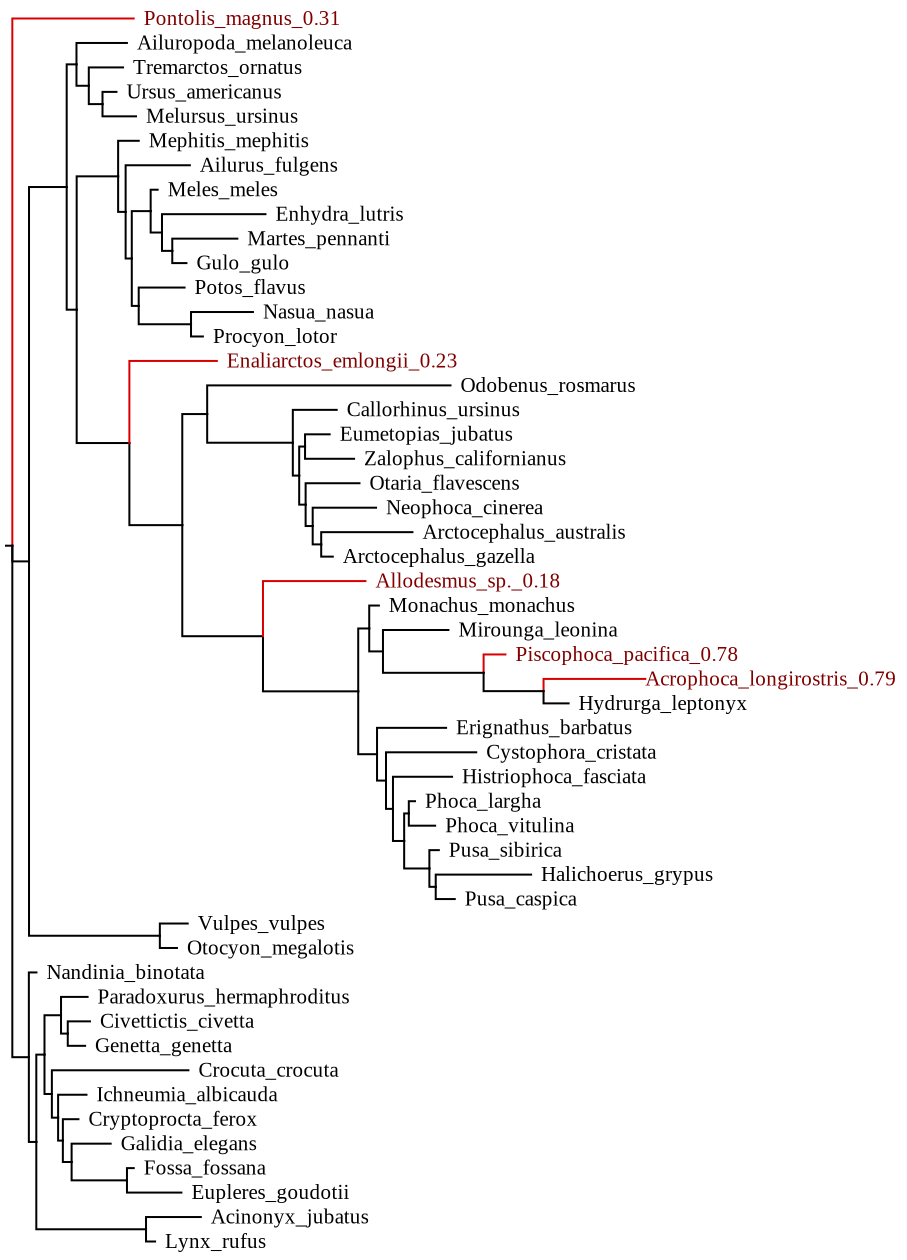
\includegraphics[width=\textwidth,height=\textheight]{/home/tomo/projects/fossil_placement/carnfig.pdf}

\textbf{Figure 3.} Fossil placements inferred from the carnivoran
dataset using the compound Dirichlet prior. Placements are displayed as
the maximum clade credibility summary of the posterior distribution of
trees. Branch lengths represent morphological disparity. Values trailing
fossil tip names display posterior support.

In both datasets, placement under the exponential branch length prior
yields conservative estimates of uncertainty in the fossil placements,
displaying generally low posterior support, except when placements are
exceptionally stable such as with \emph{Ampelocissus wildei}. This is
especially important in `rogue' taxa such as \emph{Vitis magnisperma}.
Branch support under the compound dirichlet prior is higher across several fossils in the Vitaceae dataset. The
positions of the six taxa with stable behavior (listed above) do not
change significantly under the compound dirichlet compared to the
exponential prior. Closer examination is needed to better determine the
significance of this apparent sensitivity of posterior support measures to prior choice observed in
Vitaceae. The carnivoran dataset does not exhibit the same behavior,
with both branch support and fossil placements similar across priors.

Moving forward, it will be important to explore the behavior of this
method when applied to morphometric data collected under a variety of
approaches and sampling schemes. The success of the weight calibrations
on the simulated and empirical datasets suggests the possibility of
applying the method to very large morphometric datasets by providing a
means to filter through the noise that may occur when  sampling
densely across taxa and organs. Such a framework would facilitate the
development of a more data-centric approach to morphological
phylogenetics that reduces common sources of bias in morphological 
datasets. This would encourage an exploration of conflict and
concordance in signal through quantitative data analysis rather than by
attempting to filter during the stage of data collection. They provide
a means to move forward, and should encourage the development and
exploration of more data sources to determine the most effective means
to inform phylogeny using morphometry.

It is also worth noting that certain features can be uniquely described qualitatively, such as the loss and gain of structures. 
It would be possible, and in certain cases, useful to combine such discrete information into the morphometric framework described here. This would resemble the analysis of genomic rearrangements frequently used in large molecular phylogenetic studies. As progress in this area develops, it will be important to better understand the behavior of different sources of morphological data at different timescales, and the most appropriate ways to combine, model, and gather such datasets.

\noindent\textbf{Conclusions:}

The methods described here provides a new means for biologists to
reliably and confidently place fossils in the tree of life. Although the
simulated and empirical analyses show several imperfections and a need
for further refinement of these methods, the overall accuracy and
conservative assessment of uncertainty displayed in the examples appear
encouraging. As molecular phylogenetics advances in its use of genomic
data to answer fundamental questions across the tree of life, it will be
important for morphological phylogenetics and paleontology to keep pace.
Analysis of morphometric data using the approach shown here will help to
improve issues surrounding subjectivity in character collection, and
will help morphological datasets to scale better in the genomic era. New
advances in the collection of morphometric data, combined with
refinements to the approach developed here will better equip morphology
to speak to major outstanding questions across the tree of life.


\newpage


%\bibliography{references}

\newpage

\bibliography{references}

\newpage

\end{document}